\section{Vildtforvaltning}

\begin{frame}
  \vspace{3em}
  \begin{center}
    {\LARGE \textbf{Vildtforvaltning: biotopplantiltag}
    }
    \\
    \vspace{1em}
    Bekendtgørelse om udsætning af vildt, jagtmåder og jagtredskaber
    \\
    \vspace{1em}
    BEK nr 1652 af 19/12/2017, Bilag 2
  \end{center}
\end{frame}

\begin{frame}{Biotopplaner ved udsætning af agerhøns \& fasaner}
  \begin{itemize}
    \item \textbf{Formål}: Etablere/forbedre biotoper for vildt (fugle \& pattedyr) + naturlig flora/fauna
    \item \textbf{Gennemført}: Tiltag skal være udført senest 1. juni i ansøgningsåret
    \item \textbf{Biotopplan-ejendom}: Sammenhængende arealer med samme ejer/bruger (ekskl. søer >1 ha)
    \item \textbf{Biotopplan-areal}: Non-food lavskov, dyrkede/udyrkede landbrugsarealer + udyrkede bræmmer
    \item \textbf{Krav}: Gælder kun landbrugsmæssigt dyrkede arealer
    \item Uden biotopplan: Maks. 1 fugl/ha (eller 100 stk. på <100 ha)
    \item Med biotopplan: Op til 7 fugl/ha (max 4 agerhøns/ha) ved min. point
  \end{itemize}
\end{frame}

\begin{frame}{Udsætningsgrænser \& pointkrav}
  \begin{itemize}
    \item \textbf{1-årig plan}: Min. 100 point → op til 7 fugl/ha
    \item \textbf{3-årig plan}: Min. 85 point → op til 7 fugl/ha
    \item \textbf{5-årig plan} (for 8–12 fugl/ha): Ekstra point udover basis
      \begin{itemize}
        \item 110 point → max 8 fugl/ha
        \item 120 point → max 9 fugl/ha
        \item 130 point → max 10 fugl/ha
        \item 140 point → max 11 fugl/ha
        \item 150 point → max 12 fugl/ha (max 4 agerhøns/ha)
      \end{itemize}
    \item \textbf{Særlige vilkår for 8–12/ha}: Skal have 5-årig plan + erfaring (forudgående 2 år med biotopplan)
    \item Ejendomme uden landbrugsarealer eller <22 ha dyrket areal: Op til 7 fugl/ha uden plan på ikke-dyrket del
    \item \textbf{Indberetning}: Senest 1 uge efter udsætning til Miljøstyrelsens digitale system
  \end{itemize}
\end{frame}

\begin{frame}{Krav til biotopplanens indhold \& opretholdelse}
  \begin{itemize}
    \item \textbf{Min. indhold}:
      \begin{itemize}
        \item Udpegning af arealer + tiltag på opdateret markkort (max 1:10.000)
        \item Beskrivelse + størrelse af hvert tiltag
        \item Om rævefælder forventes brugt
        \item Ansvarlig persons navn/adresse/tlf.
      \end{itemize}
    \item \textbf{Anmeldelse}: Til Miljøstyrelsen senest 1. maj (digitalt)
    \item \textbf{Opretholdelse}: Tiltag holdes i planperioden (1/3/5 år) – undtaget lærkepletter, randzoner mv. (til høst/20. feb.)
    \item \textbf{Placering}: Forbedrer naturindhold, korridorer til hegn/skove/vandløb, hensyn til mikroklima
    \item \textbf{Målrettet}: Min. 4 arter/artsgrupper (mindst 2 ikke-jagtbare)
    \item \textbf{Kontrol}: 5–10 \% stikprøver årligt af Naturstyrelsen
    \item \textbf{Kursuskrav}: Ved >100 fugl total (fasan/agerhøns/gråænder) – godkendt kursus kræves
  \end{itemize}
\end{frame}

\begin{frame}{Uddrag af pointsystemet}
  \centering
  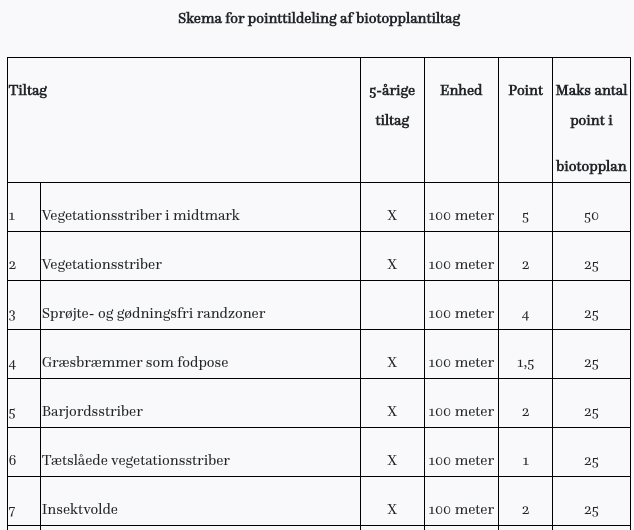
\includegraphics[width=\textwidth, height=0.8\textheight, keepaspectratio]{Billeder/Vildtforvaltning/biotopplantiltag/pointsystem.png}
\end{frame}


\begin{frame}
  \vspace{3em}
  \begin{center}
    {\LARGE \textbf{17 tiltag}
    }
    \\
    \vspace{1em}
    Jagttegnsaspiranter skal kende til 17 af pointgivende tiltag
    \\
    \vspace{1em}
    
  \end{center}
\end{frame}

% 17 tiltag til forbedringer for markvildtet

\begin{frame}{Vegetationsstriber i midtmark}

\small

\begin{columns}[T]

\begin{column}{0.58\textwidth}

\textbf{Regler ved vegetationsstriber i marken:}

\begin{itemize}[]
\item Uddyrket eller vildt- og bivenlig vegetation
\item Må ikke isås med kulturgræsser
\item Min. 3 m bred
\item Min. 40 m til kanten af det dyrkede areal
\item Må ikke gødskes eller sprøjtes
\item Ved 3- og 5-årige biotopplaner: maks. 30\% omlægges årligt
\end{itemize}

\vspace{0.4em}

\textbf{Gavner arter:}

\footnotesize
Agerhøne, fasan, hare, rådyr, dådyr, sanglærke, vibe, gul vipstjert, 
rødrygget tornskade, gulspurv, vilde bier, humlebier, 
dagsommerfugle, rovbiller, græshopper, markmus, pindsvin, lækat, flagermus, 
musvåge, tårnfalk

\end{column}

\begin{column}{0.40\textwidth}
\centering
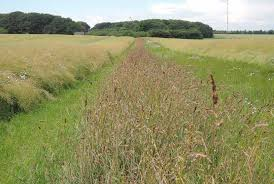
\includegraphics[width=\textwidth]{Billeder/Vildtforvaltning/biotopplantiltag/vildtstribemidtmark.jpeg}
\end{column}

\end{columns}

\end{frame}

\begin{frame}{Vegetationsstriber}

\small

\begin{columns}[T]

\begin{column}{0.58\textwidth}

\textbf{Regler ved vegetationsstriber:}

\begin{itemize}[]
\item Etableres langs søer, vandløb  og lign.
\item Uddyrket eller vildt- og bivenlig vegetation
\item Må ikke isås med kulturgræsser
\item Min. 3 m bred
\item Må ikke gødskes eller sprøjtes
\item Ved 3- og 5-årige biotopplaner: maks. 30\% af tiltaget omlægges årligt
\end{itemize}

\vspace{0.4em}

\textbf{Gavner arter:}

\footnotesize
Agerhøne, fasan, hare, rådyr, dådyr, sanglærke, vibe, gul vipstjert, 
rødrygget tornskade, gulspurv, vilde bier, humlebier, dagsommerfugle, 
rovbiller, græshopper, markmus, pindsvin, lækat, flagermus, musvåge, tårnfalk

\end{column}

\begin{column}{0.40\textwidth}
\centering
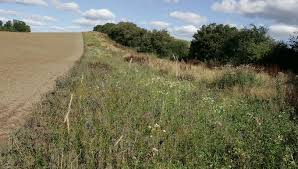
\includegraphics[width=\textwidth]{Billeder/Vildtforvaltning/biotopplantiltag/vegetationsstribe.jpeg}
\end{column}

\end{columns}

\end{frame}




\begin{frame}{Sprøjte- og gødningsfrie randzoner}

\small

\begin{columns}[T]

\begin{column}{0.58\textwidth}

\textbf{Regler ved sprøjte- og gødningsfrie randzoner:}

\begin{itemize}[]
\item Følger produktionsarealer og skal være minimum 6 m brede
\item Kan ikke placeres samme sted som andre biotopplantiltag
\item Skal opretholdes i biotopplanen fra såning og frem til høst
\end{itemize}

\vspace{0.4em}

\textbf{Gavner arter:}

\footnotesize
Vilde bier, humlebier, dagsommerfugle, svirrefluer, rovbiller, græshopper, 
gul vipstjert, sanglærke, agerhøne, vibe, rødrygget tornskade, gulspurv, 
markpiber, markmus, pindsvin, lækat, flagermus, musvåge, tårnfalk

\end{column}

\begin{column}{0.40\textwidth}
\centering
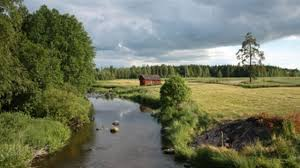
\includegraphics[width=\textwidth]{Billeder/Vildtforvaltning/biotopplantiltag/randzone.jpeg}
\end{column}

\end{columns}

\end{frame}

\begin{frame}{Græsbræmmer som fodpose}

\small

\begin{columns}[T]

\begin{column}{0.58\textwidth}

\textbf{Regler for græsbræmmer som fodpose:}

\begin{itemize}[]
\item Fodpose langs søer, vandløb, kystlinjer, vådområder, levende hegn, skovbryn, markskel og lign.
\item Består primært af græsser og urtevegetation
\item Min. 2 m bred
\item Min. 50\% soleksponeret
\item Må ikke gødskes eller sprøjtes
\end{itemize}

\vspace{0.4em}

\textbf{Gavner arter:}

\footnotesize
Agerhøne, fasan, hare, rådyr, sanglærke, vibe, gul vipstjert, rødrygget tornskade, 
gulspurv, markpiber, vilde bier, humlebier, dagsommerfugle, rovbiller, græshopper, 
overvintrende insekter, markmus, pindsvin, lækat, flagermus, musvåge, tårnfalk

\end{column}

\begin{column}{0.40\textwidth}
\centering
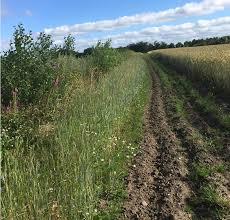
\includegraphics[width=\textwidth]{Billeder/Vildtforvaltning/biotopplantiltag/græsbræmme.jpeg}
\end{column}

\end{columns}

\end{frame}

\begin{frame}{Barjordsstriber}

\small

\begin{columns}[T]

\begin{column}{0.58\textwidth}

\textbf{Regler for barjordsstriber:}

\begin{itemize}[]
\item Udlægges langs søer, vandløb, kystlinjer, vådområder, levende hegn, skovbryn, markskel, diger, fortidsminder, beplantning, vegetationsstriber og naturarealer
\item Min. 1 m bred
\item Min. 50\% soleksponeret
\item Plantedække max. 20\% over 100 m strækning
\end{itemize}

\vspace{0.4em}

\textbf{Gavner arter:}

\footnotesize
Vibe, agerhøne, sanglærke, gul vipstjert, 
rødrygget tornskade, gulspurv, vilde bier, humlebier, dagsommerfugle, 
rovbiller, græshopper, markmus, pindsvin, lækat, musvåge, tårnfalk

\end{column}

\begin{column}{0.40\textwidth}
\centering
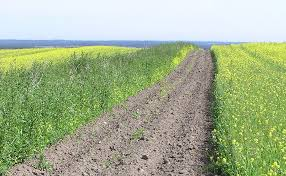
\includegraphics[width=\textwidth]{Billeder/Vildtforvaltning/biotopplantiltag/barjordsstribe.jpeg}
\end{column}

\end{columns}

\end{frame}

\begin{frame}{Tætslåede vegetationsstriber}

\small

\begin{columns}[T]

\begin{column}{0.58\textwidth}

\textbf{Regler for tætslåede vegetationsstriber:}

\begin{itemize}[]
\item Holdes kort ved hyppig slåning
\item Må ikke kunne indbyde til redeskjul
\item Min. 2 m brede
\item Max. 6 m brede
\item Min. 20 m mellem striberne
\end{itemize}

\vspace{0.4em}

\textbf{Gavner arter:}

\footnotesize
Vibe, sanglærke, markpiber, finke, agerhøne, gul vipstjert, 
rødrygget tornskade, gulspurv, vilde bier, humlebier, dagsommerfugle, 
svirrefluer, rovbiller, græshopper, markmus, pindsvin, musvåge, tårnfalk

\end{column}

\begin{column}{0.40\textwidth}
\centering
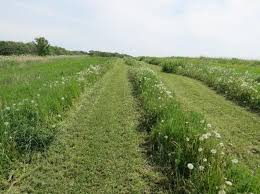
\includegraphics[width=\textwidth]{Billeder/Vildtforvaltning/biotopplantiltag/slået_vegetationsstribe.jpeg}
\end{column}

\end{columns}

\end{frame}

\begin{frame}{Insektvolde}

\small

\begin{columns}[T]

\begin{column}{0.58\textwidth}

\textbf{Regler for insektvolde:}

\begin{itemize}[]
\item Tilsås med tuegræsser
\item Min. 20 m mellem voldene
\item Min. 50\% soleksponeret
\item Skal kunne etableres og fjernes med landbrugsmaskiner
\item Min. 1 m bred
\end{itemize}

\vspace{0.4em}

\textbf{Gavner arter:}

\footnotesize
Vilde bier, humlebier, solitære bier, dagsommerfugle, svirrefluer, rovfugle, 
græshopper, overvintrende insekter, gul vipstjert, rødrygget tornskade, 
pirol, svaler, flagermus, pindsvin, lækat, musvåge, tårnfalk

\end{column}

\begin{column}{0.40\textwidth}
\centering
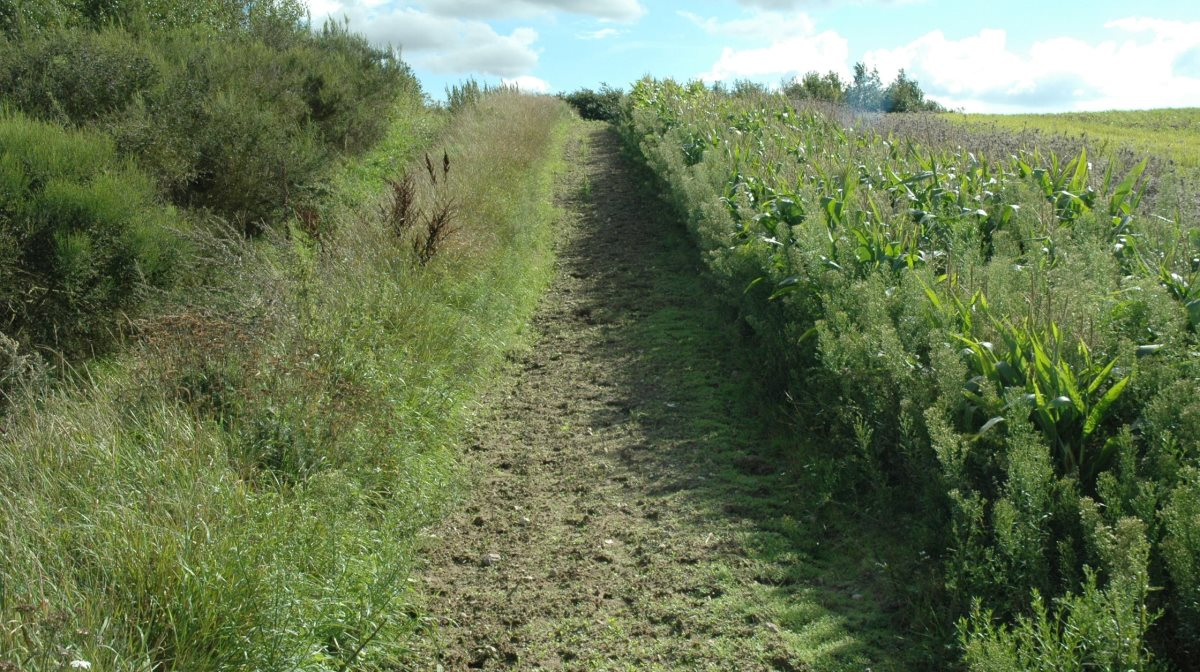
\includegraphics[width=\textwidth]{Billeder/Vildtforvaltning/biotopplantiltag/insektvold.jpg}
\end{column}

\end{columns}

\end{frame}

\begin{frame}{Kyllingestriber}

\small

\begin{columns}[T]

\begin{column}{0.58\textwidth}

\textbf{Regler for kyllingestriber:}

\begin{itemize}[]
\item Tilsås med 30\% udsædsmængde (synlig reduktion ift. tilstødende areal)
\item Minimum 3 m brede
\item Skal kombineres med tiltaget "sprøjte- og gødningsfri randzone"
\end{itemize}

\vspace{0.4em}

\textbf{Gavner arter:}

\footnotesize
Agerhøne, fasan, sanglærke, vibe, markpiber, gul vipstjert, 
rødrygget tornskade, gulspurv, agerpistol, vilde bier, humlebier, 
dagsommerfugle, rovbiller, græshopper, markmus, pindsvin, musvåge, tårnfalk

\end{column}

\begin{column}{0.40\textwidth}
\centering
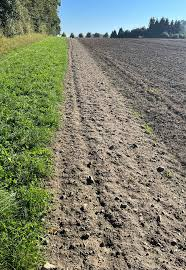
\includegraphics[width=\textwidth]{Billeder/Vildtforvaltning/biotopplantiltag/kyllingestriber.jpeg}
\end{column}

\end{columns}

\end{frame}

\begin{frame}{Lærkepletter}

\small

\begin{columns}[T]

\begin{column}{0.58\textwidth}

\textbf{Regler for lærkepletter:}

\begin{itemize}[]
\item Mindst 16 m²
\item Min. 2 per hektar
\item Mindst 40 m til kanten af marken
\item Må ikke gødskes eller sprøjtes
\end{itemize}

\vspace{0.4em}

\textbf{Gavner arter:}

\footnotesize
Sanglærke, bomlærke, vibe, agerhøne, markpiber, agerpistol, gul vipstjert, 
rødrygget tornskade, gulspurv, vilde bier, humlebier, dagsommerfugle, 
rovbiller, græshopper, musvåge, tårnfalk

\end{column}

\begin{column}{0.40\textwidth}
\centering
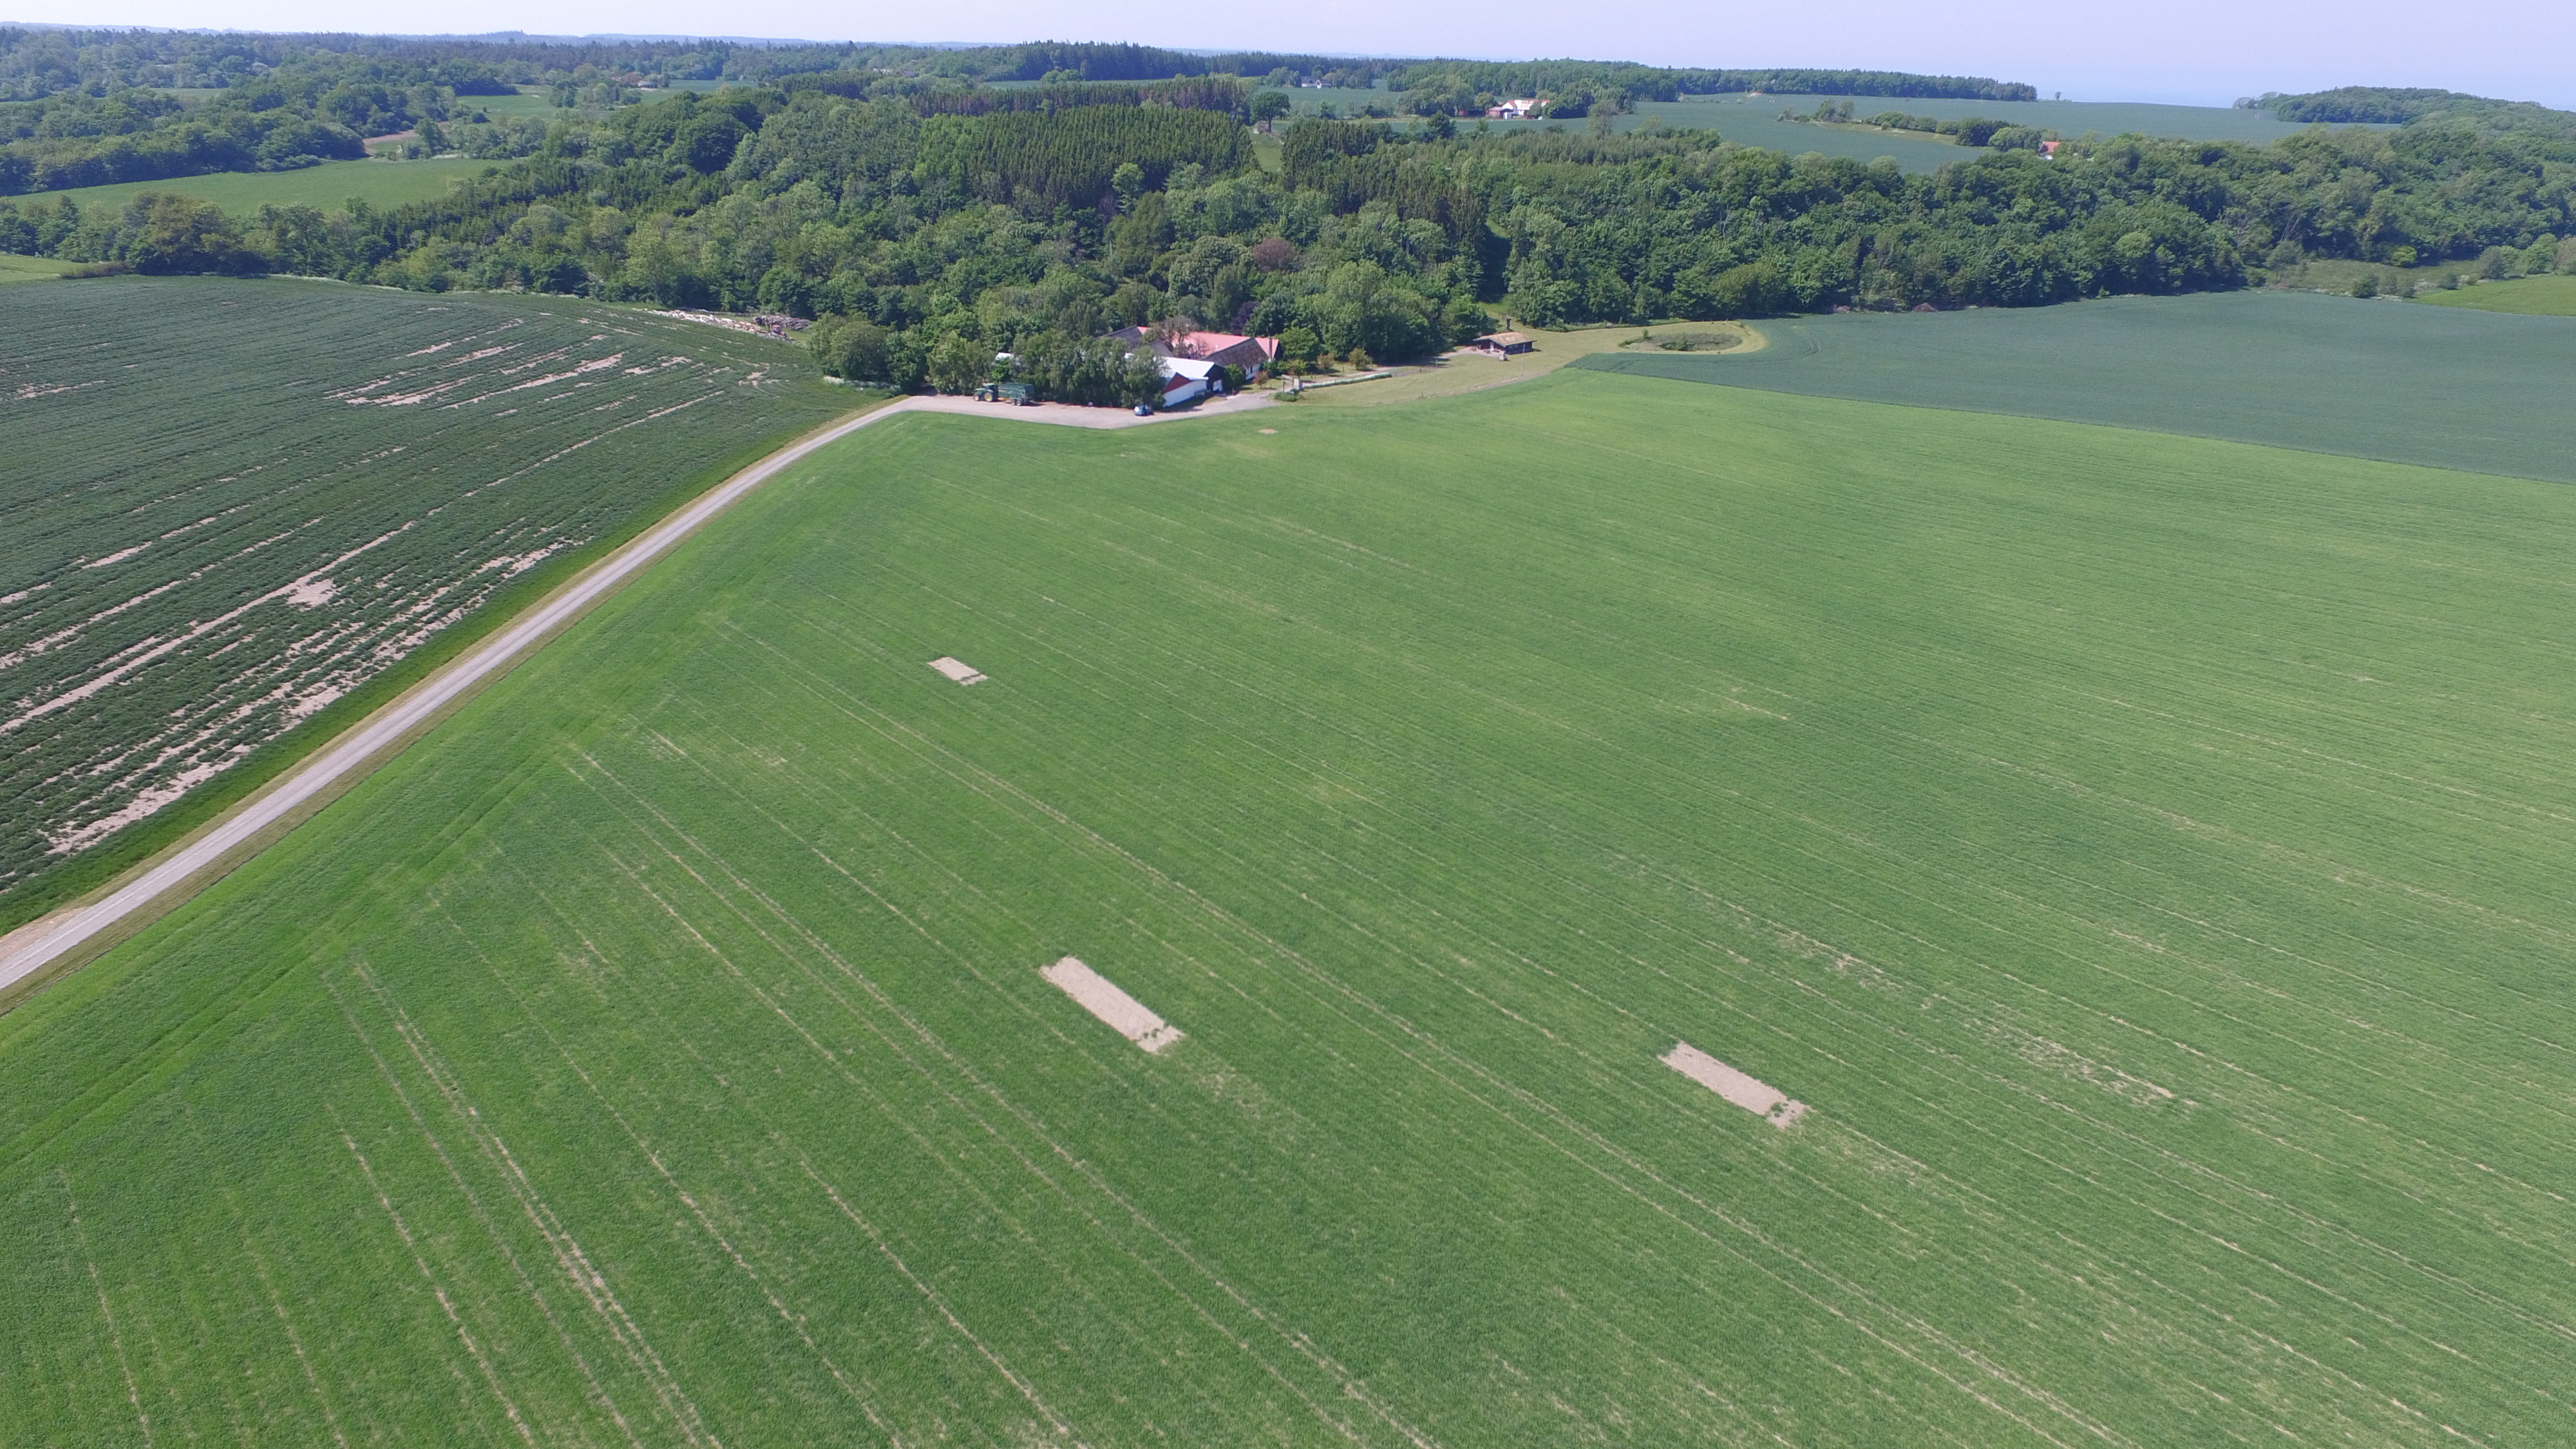
\includegraphics[width=\textwidth]{Billeder/Vildtforvaltning/biotopplantiltag/lærkepletter.jpeg}
\end{column}

\end{columns}

\end{frame}

\begin{frame}{Vibelavninger}

\small

\begin{columns}[T]

\begin{column}{0.58\textwidth}

\textbf{Regler for vibelavninger:}

\begin{itemize}[]
\item Min. 16 m²
\item Min. 1 pr. ha
\item Min. 40 m til markkant
\item Må ikke gødskes eller sprøjtes
\end{itemize}

\vspace{0.4em}

\textbf{Gavner arter:}

\footnotesize
Vibe, sanglærke, agerhøne, dobbeltbekkasin, engpiber, gul vipstjert, 
rødrygget tornskade, gulspurv, markpiber, vilde bier, humlebier, 
dagsommerfugle, rovbiller, græshopper, pindsvin, musvåge, tårnfalk

\end{column}

\begin{column}{0.40\textwidth}
\centering
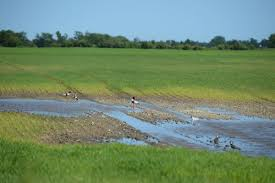
\includegraphics[width=\textwidth]{Billeder/Vildtforvaltning/biotopplantiltag/vibelavninger.jpeg}
\end{column}

\end{columns}

\end{frame}

\begin{frame}{Lysåben vegetation / arronderinger}

\small

\begin{columns}[T]

\begin{column}{0.58\textwidth}

\textbf{Regler for lysåben vegetation / arronderinger:}

\begin{itemize}[]
\item \textbf{Arrondering}: Fx afrunding af hjørner i marken
\item Kan bestå af: græsarealer, naturlig vegetation (udyrket areal) og/eller vildtstriber
\item \textbf{Græsarealer}: Primært græs, plejet kort via afgræsning eller høslet
\item \textbf{Vildtstriber}: Tilsået med vildt- og bivenlige plantearter
\item Tilladte arter: Alle ikke-traditionelle afgrøder i renbestand
\end{itemize}

\vspace{0.05em}

\textbf{Gavner arter:}

\footnotesize
Agerhøne, fasan, hare, rådyr, sanglærke, vibe, gul vipstjert, 
rødrygget tornskade, gulspurv, markpiber, vilde bier, humlebier, 
dagsommerfugle, svirrefluer, rovbiller, græshopper, markmus, 
pindsvin, lækat, flagermus, musvåge, tårnfalk

\end{column}

\begin{column}{0.40\textwidth}
\centering
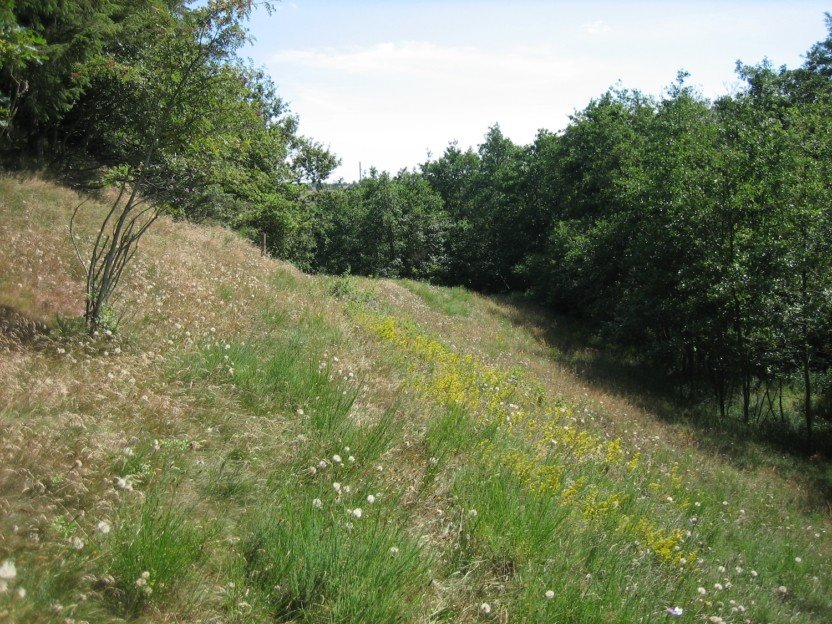
\includegraphics[width=\textwidth]{Billeder/Vildtforvaltning/biotopplantiltag/lysåben.jpg}
\end{column}

\end{columns}

\end{frame}

\begin{frame}{Stubmark og efterafgrøder}

\small

\begin{columns}[T]

\begin{column}{0.58\textwidth}

\textbf{Regler for stubmark og efterafgrøder:}

\begin{itemize}[]
\item Efterafgrøde kan være korsblomstrede afgrøder (f.eks. olieræddike, gul sennep, cikorie) eller græs og kornafgrøder
\item Efterafgrøder skal ligge vinteren over til den 20. februar
\item Min. 1 m bred
\end{itemize}

\vspace{0.4em}

\textbf{Gavner arter:}

\footnotesize
Fasan, hare, rådyr, sanglærke, agerhøne, gul vipstjert, rødrygget tornskade, 
gulspurv, agerspurv, gråspurv, markspurv, vild due, vilde bier, humlebier, 
overvintrende insekter, markmus, pindsvin, musvåge, tårnfalk, rødhals

\end{column}

\begin{column}{0.40\textwidth}
\centering
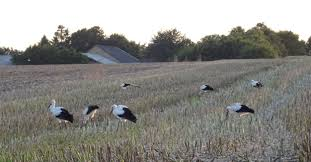
\includegraphics[width=\textwidth]{Billeder/Vildtforvaltning/biotopplantiltag/stubmark.jpeg}
% Bemærk: Jeg ændrede filnavnet til stubmark.jpg – tilpas det til dit faktiske billede
\end{column}

\end{columns}

\end{frame}

\begin{frame}{Etablering af træ- og buskbevoksninger}

\small

\begin{columns}[T]

\begin{column}{0.58\textwidth}

\textbf{Regler for etablering af træ- og buskbevoksninger:}

\begin{itemize}[]
\item Max. 0,5 ha pr. tiltag
\item Min. 50 m mellem tiltag
\end{itemize}

\vspace{0.4em}

\textbf{Gavner arter:}

\footnotesize
Fasan, agerhøne, markhare, rådyr, dådyr, rødrygget tornskade, gul vipstjert, 
pirol, gulspurv, blåmejse, musvit, sortmejse, grønsisken, stillits, 
rødhals, flagermus, pindsvin, lækat, egern, musvåge, spurvehøg, tårnfalk

\end{column}

\begin{column}{0.40\textwidth}
\centering
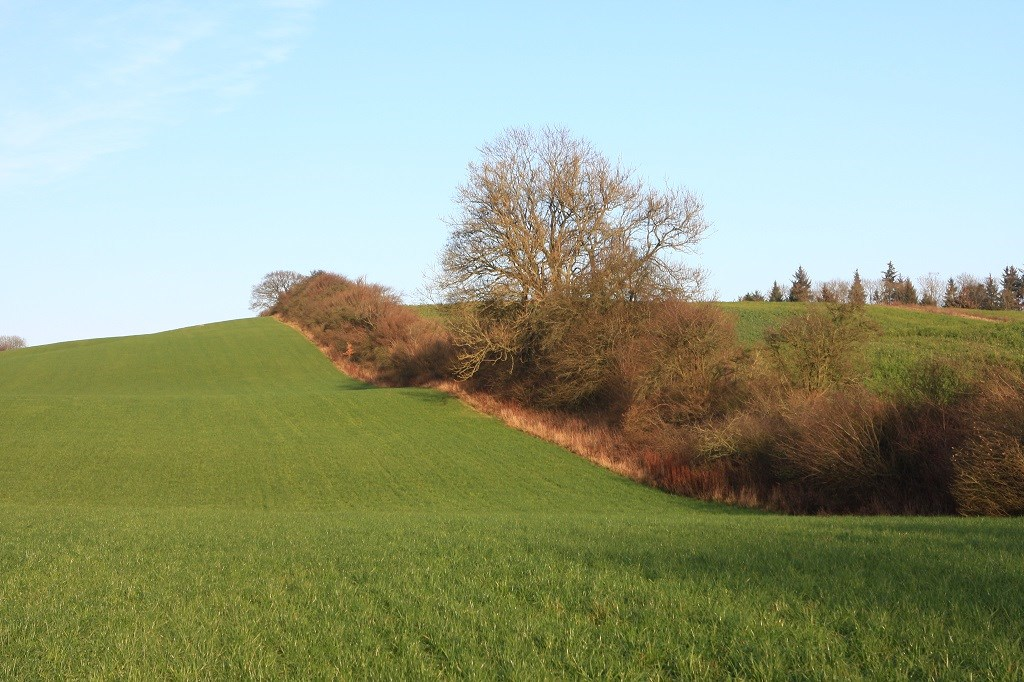
\includegraphics[width=\textwidth]{Billeder/Vildtforvaltning/biotopplantiltag/buskbevoksning.jpg}
\end{column}

\end{columns}

\end{frame}

\begin{frame}{Etablering af levende hegn og linieformede markopdelinger}

\small

\begin{columns}[T]

\begin{column}{0.58\textwidth}

\textbf{Regler for etablering af levende hegn og linieformede markopdelinger:}

\begin{itemize}[]
\item Min. 2 m bred
\item Anlægges langs grøfter, diger, veje mm.
\item Ved mere end tre rækker: lysåbning hver 50. meter
\end{itemize}

\vspace{0.4em}

\textbf{Gavner arter:}

\footnotesize
Fasan, agerhøne, markhare, rådyr, dådyr, rødrygget tornskade, gul vipstjert, 
pirol, gulspurv, blåmejse, musvit, sortmejse, grønsisken, stillits, rødhals, 
nattergal, hærfugl, flagermus, pindsvin, lækat, egern, musvåge, spurvehøg, 
tårnfalk, rørhøg

\end{column}

\begin{column}{0.40\textwidth}
\centering
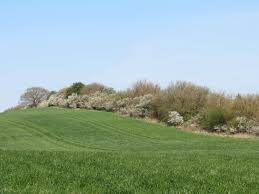
\includegraphics[width=\textwidth]{Billeder/Vildtforvaltning/biotopplantiltag/levendehegn.jpeg}
\end{column}

\end{columns}

\end{frame}

\begin{frame}{Levende hegn og linieformede markopdelinger}

\small

\begin{columns}[T]

\begin{column}{0.58\textwidth}

\textbf{Regler for levende hegn og linieformede markopdelinger:}

\begin{itemize}[]
\item Min. 2 m bred
\item Min. 75\% hjemmehørende arter efter 10 år
\item Skal løbende plejes med beskæring
\item Skal suppleres for at opnå point
\end{itemize}

\vspace{0.4em}

\textbf{Gavner arter:}

\footnotesize
Fasan, agerhøne, markhare, rådyr, dådyr, rødrygget tornskade, gul vipstjert, 
pirol, gulspurv, blåmejse, musvit, sortmejse, grønsisken, stillits, rødhals, 
nattergal, hærfugl, flagermus, pindsvin, lækat, egern, musvåge, spurvehøg, 
tårnfalk, rørhøg

\end{column}

\begin{column}{0.40\textwidth}
\centering
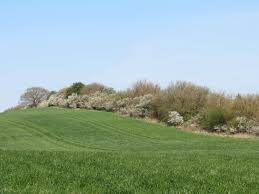
\includegraphics[width=\textwidth]{Billeder/Vildtforvaltning/biotopplantiltag/levendehegn.jpeg}
\end{column}

\end{columns}

\end{frame}

\begin{frame}{Etablering af skov}

\small

\begin{columns}[T]

\begin{column}{0.58\textwidth}

\textbf{Regler for etablering af skov:}

\begin{itemize}[]
\item Opfylder regler for skovrejsning
\item Skal opfylde kravene for tilskud under skovrejsningsordningerne
\item Tiltaget er pointgivende i 5 år fra anlæggelsesåret
\end{itemize}

\vspace{0.4em}

\textbf{Gavner arter:}

\footnotesize
Rådyr, dådyr, ræv, hare, fasan, rødrygget tornskade, gul vipstjert, 
pirol, gulspurv, blåmejse, musvit, sortmejse, grønsisken, stillits, rødhals, 
nattergal, hærfugl, flagermus, pindsvin, lækat, egern, musvåge, spurvehøg, 
tårnfalk, rørhøg, rådyr, kronvildt (senere stadier)

\end{column}

\begin{column}{0.40\textwidth}
\centering
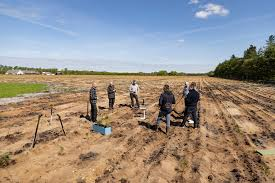
\includegraphics[width=\textwidth]{Billeder/Vildtforvaltning/biotopplantiltag/skovrejsning.jpeg}
\end{column}

\end{columns}

\end{frame}

\begin{frame}{Etablering af søer}

\small

\begin{columns}[T]

\begin{column}{0.58\textwidth}

\textbf{Regler for etablering af søer:}

\begin{itemize}[]
\item Min. 600 m²
\item Minimum 10 m bufferzone
\item Min. 50\% af bufferzonen skal være soleksponeret
\item Pointgivende i 5 år fra anlæggelsestidspunktet
\end{itemize}

\vspace{0.4em}

\textbf{Gavner arter:}

\footnotesize
Vibe, engsnarreskade, dobbeltbekkasin, rødbenet klire, gul vipstjert, 
sanglærke, agerhøne, gråstrubet lappedykker, gråand, krikand, 
padder (frøer, tudser, salamandere), guldsmed, libeller, 
vilde bier (kant), humlebier, markmus, pindsvin, flagermus, 
musvåge, tårnfalk, rørhøg

\end{column}

\begin{column}{0.40\textwidth}
\centering
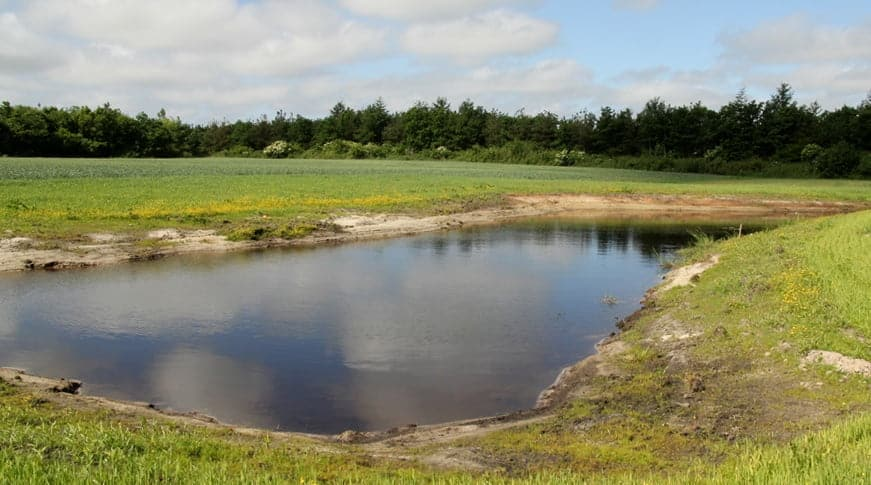
\includegraphics[width=\textwidth]{Billeder/Vildtforvaltning/biotopplantiltag/etableringafsø.jpg}
\end{column}

\end{columns}

\end{frame}